\documentclass[border=10pt, tikz]{standalone}

\usetikzlibrary{
    positioning,
    arrows.meta,
    calc,
    backgrounds,
    decorations.markings,
    fit,
    shapes.geometric
}

\usepackage{amsmath, amssymb}
\usepackage{xcolor}

% ============================================
% PALETTE
% ============================================
\definecolor{accent}{HTML}{E07B54}
\definecolor{encoder}{HTML}{5DADE2}
\definecolor{encoderdark}{HTML}{2E86C1}
\definecolor{attention}{HTML}{AF7AC5}
\definecolor{attentiondark}{HTML}{884EA0}
\definecolor{drift}{HTML}{58D68D}
\definecolor{driftdark}{HTML}{28B463}
\definecolor{gate}{HTML}{F4D03F}
\definecolor{gatedark}{HTML}{D4AC0D}

\definecolor{recv}{HTML}{E74C3C}
\definecolor{spatial}{HTML}{5DADE2}
\definecolor{refcol}{HTML}{58D68D}

\definecolor{blockbg}{HTML}{F5F7FA}
\definecolor{blockline}{HTML}{B0B8C0}
\definecolor{textmain}{HTML}{1A1A2E}
\definecolor{textsub}{HTML}{5A6070}

% ============================================
% STYLES
% ============================================
\tikzset{
    % Shadowed blocks for multi-head
    shadowed/.style={
        preaction={fill=#1!12, transform canvas={xshift=1.8pt, yshift=-1.8pt}},
        preaction={fill=#1!22, transform canvas={xshift=0.9pt, yshift=-0.9pt}},
        fill=#1!32
    },
    % Layer blocks
    layer/.style={
        rectangle, rounded corners=2mm,
        minimum height=2em, minimum width=2.8cm,
        draw=#1!70, line width=0.5pt, fill=#1!18,
        font=\fontsize{7}{8}\selectfont\sffamily, text=textmain
    },
    layersmall/.style={
        rectangle, rounded corners=1.5mm,
        minimum height=1.6em, minimum width=1.6cm,
        draw=#1!70, line width=0.4pt, fill=#1!18,
        font=\fontsize{6}{7}\selectfont\sffamily, text=textmain
    },
    % Multi-head block
    mhblock/.style={
        rectangle, rounded corners=2mm,
        minimum height=2.2em, minimum width=3cm,
        draw=#1!70, line width=0.5pt, shadowed=#1,
        font=\fontsize{7}{8}\selectfont\sffamily, text=textmain
    },
    % Background block
    bgblock/.style={
        rectangle, rounded corners=4mm,
        fill=blockbg, draw=blockline, line width=0.4pt
    },
    % Circles
    iocircle/.style={
        circle, minimum size=2.4em,
        draw=#1!70, fill=#1!22, line width=0.5pt,
        font=\fontsize{7}{8}\selectfont\sffamily
    },
    % Tokens
    tok/.style={
        rectangle, rounded corners=1pt,
        fill=#1!40, draw=#1!60,
        minimum height=5.5mm, minimum width=5.5mm, line width=0.35pt
    },
    % Matrix
    matrixbox/.style={
        rectangle, rounded corners=1mm,
        fill=#1!12, draw=#1!45, line width=0.4pt
    },
    % Panel
    panel/.style={
        rectangle, rounded corners=5pt,
        fill=white, draw=blockline, line width=0.5pt
    },
    % Text styles
    title/.style={font=\fontsize{10}{11}\selectfont\bfseries\sffamily, text=textmain},
    subtitle/.style={font=\fontsize{7}{8}\selectfont\sffamily, text=textsub},
    annot/.style={font=\fontsize{6}{7}\selectfont\sffamily, text=textsub},
    dim/.style={font=\fontsize{5.5}{6.5}\selectfont\sffamily, text=textsub},
    math/.style={font=\fontsize{7}{8}\selectfont, text=textsub},
    % Arrows
    arr/.style={-{Stealth[length=1.8mm, width=1.3mm]}, line width=0.45pt, draw=textsub},
    arrthick/.style={-{Stealth[length=2mm, width=1.5mm]}, line width=0.6pt, draw=textsub},
    arraccent/.style={-{Stealth[length=2.2mm, width=1.6mm]}, line width=0.7pt, draw=accent},
    skip/.style={-latex, line width=0.4pt, draw=textsub!50, rounded corners=2mm},
}

\begin{document}
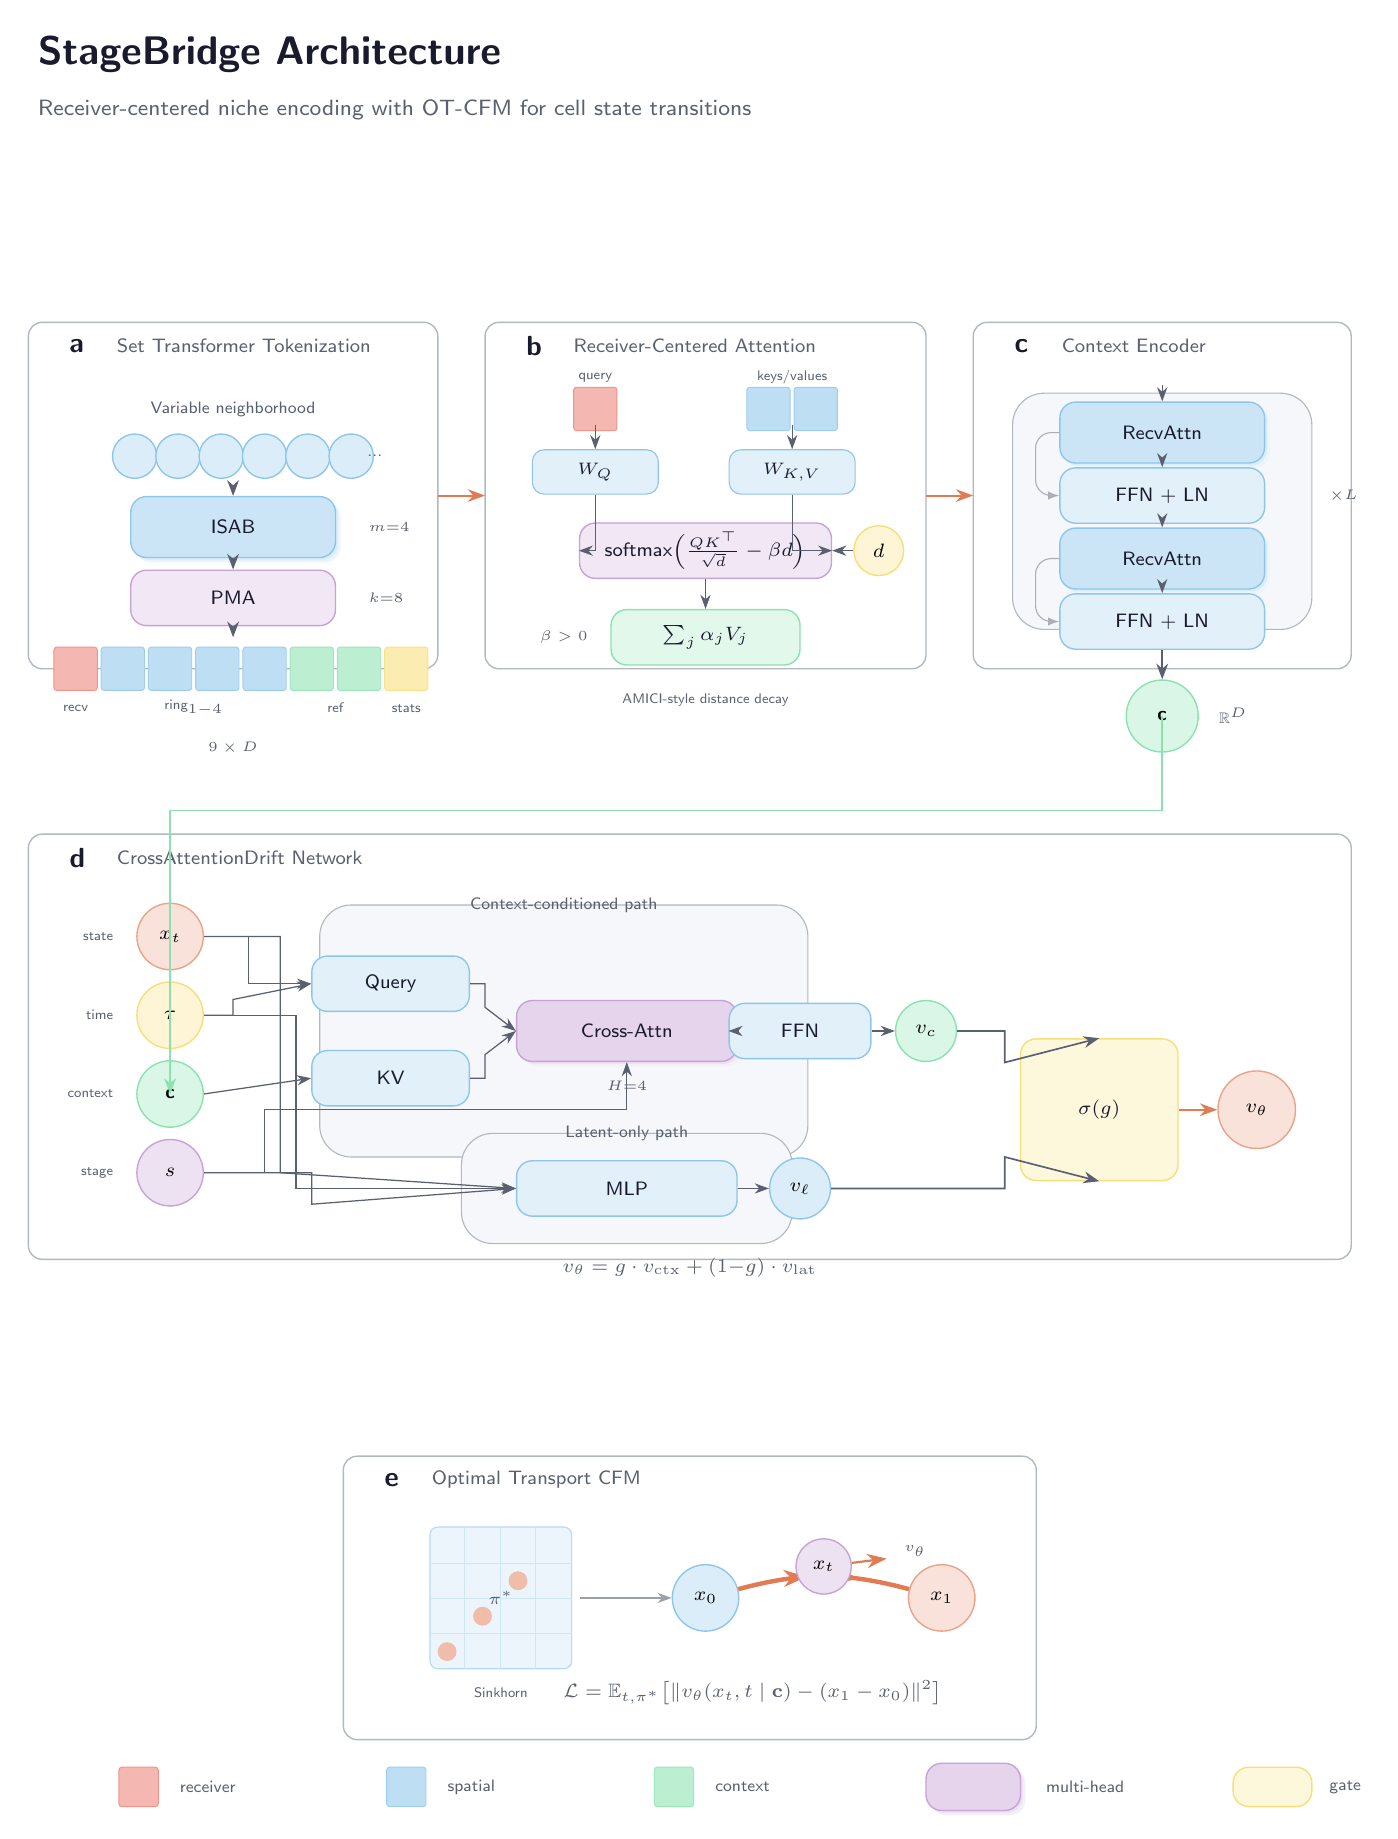
\begin{tikzpicture}[x=1mm, y=1mm]

% ============================================
% HEADER
% ============================================
\node[font=\fontsize{14}{16}\selectfont\bfseries\sffamily, text=textmain, anchor=west]
    at (0, 118) {StageBridge Architecture};
\node[font=\fontsize{8}{9}\selectfont\sffamily, text=textsub, anchor=west]
    at (0, 111) {Receiver-centered niche encoding with OT-CFM for cell state transitions};

% ============================================
% a) TOKENIZATION
% ============================================
\begin{scope}[shift={(0, 62)}]
    \node[panel, minimum width=52mm, minimum height=44mm] at (26, 0) {};
    \node[title, anchor=west] at (4, 19) {a};
    \node[subtitle, anchor=west] at (10, 19) {Set Transformer Tokenization};

    % Variable input
    \node[annot] at (26, 11) {Variable neighborhood};
    \foreach \i in {1,...,6} {
        \node[iocircle=spatial, minimum size=1.6em] at ({8 + \i*5.5}, 5) {};
    }
    \node[annot] at (44, 5) {...};

    % ISAB
    \node[mhblock=encoder, minimum width=2.6cm] (isab) at (26, -4) {ISAB};
    \node[dim, anchor=west] at (42, -4) {$m{=}4$};

    % PMA
    \node[layer=attention, minimum width=2.6cm] (pma) at (26, -13) {PMA};
    \node[dim, anchor=west] at (42, -13) {$k{=}8$};

    \draw[arrthick] (26, 1) -- (isab);
    \draw[arrthick] (isab) -- (pma);

    % Output tokens
    \node[tok=recv] at (6, -22) {};
    \node[tok=spatial] at (12, -22) {};
    \node[tok=spatial] at (18, -22) {};
    \node[tok=spatial] at (24, -22) {};
    \node[tok=spatial] at (30, -22) {};
    \node[tok=refcol] at (36, -22) {};
    \node[tok=refcol] at (42, -22) {};
    \node[tok=gate] at (48, -22) {};

    \node[dim] at (6, -27) {recv};
    \node[dim] at (21, -27) {ring$_{1-4}$};
    \node[dim] at (39, -27) {ref};
    \node[dim] at (48, -27) {stats};

    \draw[arrthick] (pma) -- (26, -18);

    \node[dim] at (26, -32) {$9 \times D$};
\end{scope}

% ============================================
% b) RECEIVER-CENTERED ATTENTION
% ============================================
\begin{scope}[shift={(58, 62)}]
    \node[panel, minimum width=56mm, minimum height=44mm] at (28, 0) {};
    \node[title, anchor=west] at (4, 19) {b};
    \node[subtitle, anchor=west] at (10, 19) {Receiver-Centered Attention};

    % Tokens
    \node[tok=recv] at (14, 11) {};
    \node[dim] at (14, 15) {query};

    \node[tok=spatial] at (36, 11) {};
    \node[tok=spatial] at (42, 11) {};
    \node[dim] at (39, 15) {keys/values};

    % Projections
    \node[layersmall=encoder] (wq) at (14, 3) {$W_Q$};
    \node[layersmall=encoder] (wkv) at (39, 3) {$W_{K,V}$};

    \draw[arr] (14, 9) -- (wq);
    \draw[arr] (39, 9) -- (wkv);

    % Attention with distance
    \node[layer=attention, minimum width=3.2cm] (attn) at (28, -7) {$\text{softmax}\!\left(\frac{QK^\top}{\sqrt{d}} - \beta d\right)$};

    \draw[arr] (wq) -- (14, -7) -- (attn.west);
    \draw[arr] (wkv) -- (39, -7) -- (attn.east);

    % Distance input
    \node[iocircle=gate, minimum size=1.8em] (dist) at (50, -7) {$d$};
    \draw[arr] (dist) -- (attn);

    % Output
    \node[layer=drift, minimum width=2.4cm] (out) at (28, -18) {$\sum_j \alpha_j V_j$};
    \draw[arr] (attn) -- (out);

    % Beta note
    \node[dim] at (10, -18) {$\beta > 0$};

    \node[dim] at (28, -26) {AMICI-style distance decay};
\end{scope}

% Arrow a->b
\draw[arraccent] (52, 62) -- (58, 62);

% ============================================
% c) CONTEXT ENCODER
% ============================================
\begin{scope}[shift={(120, 62)}]
    \node[panel, minimum width=48mm, minimum height=44mm] at (24, 0) {};
    \node[title, anchor=west] at (4, 19) {c};
    \node[subtitle, anchor=west] at (10, 19) {Context Encoder};

    % Encoder block
    \node[bgblock, minimum width=38mm, minimum height=30mm] at (24, -2) {};

    % Layers
    \node[mhblock=encoder, minimum width=2.6cm] (l1) at (24, 8) {RecvAttn};
    \node[layer=encoder, minimum width=2.6cm] (ffn1) at (24, 0) {FFN + LN};
    \node[mhblock=encoder, minimum width=2.6cm] (l2) at (24, -8) {RecvAttn};
    \node[layer=encoder, minimum width=2.6cm] (ffn2) at (24, -16) {FFN + LN};

    \draw[arr] (24, 14) -- (l1);
    \draw[arr] (l1) -- (ffn1);
    \draw[arr] (ffn1) -- (l2);
    \draw[arr] (l2) -- (ffn2);

    % Skip connections
    \draw[skip] (l1.west) -- ++(-3,0) |- (ffn1.west);
    \draw[skip] (l2.west) -- ++(-3,0) |- (ffn2.west);

    \node[dim, anchor=west] at (44, 0) {$\times L$};

    % Output
    \node[iocircle=refcol, minimum size=2.6em] (ctx) at (24, -28) {\textbf{c}};
    \draw[arrthick] (ffn2) -- (ctx);
    \node[dim, anchor=west] at (30, -28) {$\mathbb{R}^D$};
\end{scope}

% Arrow b->c
\draw[arraccent] (114, 62) -- (120, 62);

% ============================================
% d) CROSS-ATTENTION DRIFT
% ============================================
\begin{scope}[shift={(0, -8)}]
    \node[panel, minimum width=168mm, minimum height=54mm] at (84, 0) {};
    \node[title, anchor=west] at (4, 24) {d};
    \node[subtitle, anchor=west] at (10, 24) {CrossAttentionDrift Network};

    % Inputs
    \node[iocircle=accent] (xt) at (18, 14) {$x_t$};
    \node[iocircle=gate] (temb) at (18, 4) {$\tau$};
    \node[iocircle=refcol] (ctx) at (18, -6) {\textbf{c}};
    \node[iocircle=attention] (stg) at (18, -16) {$s$};

    \node[dim, anchor=east] at (12, 14) {state};
    \node[dim, anchor=east] at (12, 4) {time};
    \node[dim, anchor=east] at (12, -6) {context};
    \node[dim, anchor=east] at (12, -16) {stage};

    % Context path background
    \node[bgblock, minimum width=62mm, minimum height=32mm] at (68, 2) {};
    \node[annot] at (68, 18) {Context-conditioned path};

    % Query proj
    \node[layer=encoder, minimum width=2cm] (qproj) at (46, 8) {Query};
    \draw[arr] (xt.east) -- (28, 14) -- (28, 8) -- (qproj.west);
    \draw[arr] (temb.east) -- (26, 4) -- (26, 6) -- (qproj.west);

    % KV proj
    \node[layer=encoder, minimum width=2cm] (kvproj) at (46, -4) {KV};
    \draw[arr] (ctx.east) -- (kvproj.west);

    % Cross attention
    \node[mhblock=attention, minimum width=2.8cm] (mha) at (76, 2) {Cross-Attn};
    \node[dim] at (76, -5) {$H{=}4$};

    \draw[arr] (qproj.east) -- (58, 8) -- (58, 5) -- (mha.west);
    \draw[arr] (kvproj.east) -- (58, -4) -- (58, -1) -- (mha.west);
    \draw[arr] (stg.east) -- (30, -16) -- (30, -8) -- (76, -8) -- (mha.south);

    % FFN
    \node[layer=encoder, minimum width=1.8cm] (ffn) at (98, 2) {FFN};
    \draw[arr] (mha) -- (ffn);

    % v_ctx output
    \node[iocircle=refcol, minimum size=2.2em] (vctx) at (114, 2) {$v_c$};
    \draw[arr] (ffn) -- (vctx);

    % Latent path background
    \node[bgblock, minimum width=42mm, minimum height=14mm] at (76, -18) {};
    \node[annot] at (76, -11) {Latent-only path};

    % MLP
    \node[layer=encoder, minimum width=2.8cm] (mlp) at (76, -18) {MLP};
    \draw[arr] (xt.east) -- (32, 14) -- (32, -16) -- (mlp.west);
    \draw[arr] (temb.east) -- (34, 4) -- (34, -18) -- (mlp.west);
    \draw[arr] (stg.east) -- (36, -16) -- (36, -20) -- (mlp.west);

    % v_lat output
    \node[iocircle=encoder, minimum size=2.2em] (vlat) at (98, -18) {$v_\ell$};
    \draw[arr] (mlp) -- (vlat);

    % Gate
    \node[layer=gate, minimum width=2cm, minimum height=1.8cm] (gblock) at (136, -8) {$\sigma(g)$};

    \draw[arrthick] (vctx.east) -- (124, 2) -- (124, -2) -- (gblock.north);
    \draw[arrthick] (vlat.east) -- (110, -18) -- (124, -18) -- (124, -14) -- (gblock.south);

    % Output
    \node[iocircle=accent, minimum size=2.8em] (vout) at (156, -8) {$v_\theta$};
    \draw[arraccent] (gblock) -- (vout);

    % Equation
    \node[math] at (84, -28) {$v_\theta = g \cdot v_{\text{ctx}} + (1{-}g) \cdot v_{\text{lat}}$};
\end{scope}

% Context connection
\draw[arrthick, draw=refcol!70] (144, 34) -- (144, 22) -| (18, -14);

% ============================================
% e) OT-CFM
% ============================================
\begin{scope}[shift={(40, -78)}]
    \node[panel, minimum width=88mm, minimum height=36mm] at (44, 0) {};
    \node[title, anchor=west] at (4, 15) {e};
    \node[subtitle, anchor=west] at (10, 15) {Optimal Transport CFM};

    % Coupling matrix
    \node[matrixbox=spatial, minimum width=18mm, minimum height=18mm] (coup) at (20, 0) {};
    \foreach \i in {1,...,3} {
        \draw[spatial!30, line width=0.3pt] ($(coup.south west) + (\i*4.5mm, 0)$) -- ($(coup.north west) + (\i*4.5mm, 0)$);
        \draw[spatial!30, line width=0.3pt] ($(coup.south west) + (0, \i*4.5mm)$) -- ($(coup.south east) + (0, \i*4.5mm)$);
    }
    \foreach \i in {1,...,3} {
        \fill[accent!50] ($(coup.south west) + (\i*4.5mm - 2.25mm, \i*4.5mm - 2.25mm)$) circle (1.2mm);
    }
    \node[annot] at (20, 0) {$\pi^*$};
    \node[dim] at (20, -12) {Sinkhorn};

    % Source/target
    \node[iocircle=spatial, minimum size=2.4em] (x0) at (46, 0) {$x_0$};
    \node[iocircle=accent, minimum size=2.4em] (x1) at (76, 0) {$x_1$};

    % Trajectory
    \draw[line width=1.6pt, accent,
        postaction={decorate, decoration={markings,
            mark=at position 0.4 with {\arrow[accent, scale=0.8]{Stealth}},
            mark=at position 0.7 with {\arrow[accent, scale=0.8]{Stealth}}}}
    ] (x0) to[out=15, in=165] (x1);

    % Intermediate
    \node[iocircle=attention, minimum size=2em] (xtmid) at (61, 4) {$x_t$};

    % Velocity
    \draw[-{Stealth[length=2.5mm, width=1.8mm]}, accent, line width=0.8pt] (xtmid) -- ++(8, 1);
    \node[dim, anchor=west] at (70, 6) {$v_\theta$};

    % Coupling arrow
    \draw[arr, draw=textsub!60] (30, 0) -- (x0);

    % Loss
    \node[math] at (52, -12) {$\mathcal{L} = \mathbb{E}_{t, \pi^*}\!\left[\|v_\theta(x_t, t \mid \mathbf{c}) - (x_1 - x_0)\|^2\right]$};
\end{scope}

% ============================================
% LEGEND
% ============================================
\begin{scope}[shift={(0, -102)}]
    \node[tok=recv, minimum size=5mm] at (14, 0) {};
    \node[annot, anchor=west] at (18, 0) {receiver};

    \node[tok=spatial, minimum size=5mm] at (48, 0) {};
    \node[annot, anchor=west] at (52, 0) {spatial};

    \node[tok=refcol, minimum size=5mm] at (82, 0) {};
    \node[annot, anchor=west] at (86, 0) {context};

    \node[mhblock=attention, minimum width=1.2cm, minimum height=0.6cm] at (120, 0) {};
    \node[annot, anchor=west] at (128, 0) {multi-head};

    \node[layer=gate, minimum width=1cm, minimum height=0.5cm] at (158, 0) {};
    \node[annot, anchor=west] at (164, 0) {gate};
\end{scope}

\end{tikzpicture}
\end{document}
